\documentclass{article}

% Camera-ready: \usepackage[final]{neurips_2024}
% Preprint:     \usepackage[preprint]{neurips_2024}
\usepackage[preprint]{neurips_2024}

\usepackage[utf8]{inputenc}
\usepackage[T1]{fontenc}
\usepackage{hyperref}
\usepackage{url}
\usepackage{booktabs}
\usepackage{amsfonts, amsmath, amssymb}
\usepackage{nicefrac}
\usepackage{microtype}
\usepackage{xcolor}
\usepackage{enumitem}
\usepackage{tikz}
\usepackage{pgfplots}
\pgfplotsset{compat=1.18}

\title{The Pareto Landscape of Moral Reasoning}

\author{%
  Pierre Beckmann\\
  University of Bern\\
  \texttt{pierrebeckmann@gmail.com}
}

\begin{document}

\maketitle

\begin{abstract}
Evaluating moral reasoning is hard because the moral domain lacks the ground
truth that organises evaluation elsewhere: competent reasoners can start from
similar intuitions and reach different defensible conclusions. We argue that
this is not a measurement failure but a structural feature, and we propose a
conceptual framework that takes it seriously. Moral reasoning, on our account,
aims at a \emph{good epistemic state}: a pair of commitments and principles
that hangs together. Such a state is graded along two axis families that
genuinely conflict: epistemic desiderata (account, systematicity, faithfulness)
and value loadings (freedom, well-being, justice, dignity, solidarity). The
rational object of study is then the \emph{Pareto frontier} of attainable
epistemic states. We develop a vocabulary for the shapes this frontier takes
(convex segments, concave segments, knees, plateaus, corner attractors,
dominated regions), and we recast familiar reasoning methods --- reflective
equilibrium foremost among them --- as strategies for navigating the
landscape toward the frontier. We sketch the corpus that would let this
framework be studied empirically, and outline what such study would reveal
about moral reasoning in humans and in language models.
\end{abstract}


\section{Motivation}
\label{sec:motivation}

Current alignment work focuses on the moral \emph{content} a model holds:
constitutional principles, character training, value specifications. Less
attention has gone to moral reasoning as a \emph{capacity}~\citep{carlsmith2026}.
But a value-aligned model whose reasoning fails when its values come into
tension is still unsafe: it can produce outputs that look like principled
moral thought without being so. Diagnosing such failures is hard because the
moral domain lacks a ground truth against which to score answers
\citep{queloz2025}: competent reasoners can reach different conclusions
without either being simply wrong.

This paper proposes a framework that takes the absence of ground truth as a
\emph{structural feature} rather than a measurement failure. We articulate
what moral reasoning aims at, what makes its outputs better or worse without
a single right answer, and how the multi-objective optimisation literature
gives us a precise vocabulary for the kinds of trade-offs the moral domain
actually exhibits. Familiar methods such as reflective equilibrium then
reappear as \emph{strategies for navigating} this landscape, comparable in
principle to alternative strategies and amenable to empirical study once a
suitable corpus is in place.


\section{Conceptualising moral reasoning}
\label{sec:concept}

An \textbf{ethical situation} confronts an agent with a decision: several
actions are open, and none is clearly right or wrong. Moral reasoning is what
the agent does between encountering the situation and acting. We decompose
it into identifiable stages:

\begin{enumerate}[leftmargin=*, itemsep=2pt]
  \item \emph{Identify ethically relevant properties} of the situation ---
    who is affected, which interests are at stake, the nature of the action
    on offer.
  \item \emph{Form initial commitments} about how to act, on the basis of
    those properties. These are the agent's pre-theoretical verdicts about
    the case, the starting material of further reasoning.
  \item \emph{Propose principles}: generalise across one's commitments and
    find rules that would justify them. This is the inductive or abductive
    move.
  \item \emph{Deduce}: from a candidate principle, derive the commitments it
    would imply across other situations.
  \item \emph{Revise} when principle and commitment conflict, in either
    direction --- the dialectical move at the heart of reflective
    equilibrium~\citep{rawls1971, beisbart2021}.
  \item \emph{Evaluate} the resulting pair of commitments and principles.
\end{enumerate}

The output of moral reasoning is an \textbf{epistemic state} $\sigma = (C, P)$:
a set of commitments and a set of principles that hang together. We take the
goal of moral reasoning to be reaching a \emph{good} epistemic state. The
question is what \emph{good} means in a domain without a single right
answer.


\section{What makes an epistemic state good}
\label{sec:good}

Two axis families grade $\sigma$ simultaneously. They genuinely conflict, in
the sense that improving one typically costs another.

\paragraph{Epistemic axes.} Properties of $\sigma$ as reasoning, drawn from
the formal account of \citet{beisbart2021}.
\begin{itemize}[leftmargin=*, itemsep=2pt]
  \item \textsc{Account}: how much the principles in $P$ entail or support
    the commitments in $C$, penalising contradictions, gaps, and surplus
    content.
  \item \textsc{Systematicity}: how simple, unifying, and broadly applicable
    $P$ is, as opposed to a hodgepodge of case-by-case stipulations.
  \item \textsc{Faithfulness}: how well the current commitments respect the
    agent's initial intuitions $C_0$, penalising arbitrary drift.
\end{itemize}

\paragraph{Ethical axes.} Properties of $\sigma$ as a moral stance. Each
principle $p \in P$ carries a fuzzy \emph{value loading} $\boldsymbol{v}(p)
\in [0, 1]^K$ over a small set of basic moral values --- we work with five:
\textsc{freedom}, \textsc{well-being}, \textsc{justice}, \textsc{dignity},
and \textsc{solidarity}, chosen so that the central tensions of moral life
(liberty vs.\ community, fairness vs.\ welfare, welfare vs.\ dignity) appear
directly as trade-offs among axes. The state $\sigma$ inherits an aggregate
value position $V(\sigma) \in [0, 1]^K$.

\paragraph{Two families, two axes of disagreement.} The epistemic family is
broadly agent-independent: every reasoner has some stake in coherence. The
ethical family is agent-dependent: different agents weight different values,
and this pluralism is a constitutive feature of the moral domain rather than
noise to be averaged out. A \emph{good} epistemic state must do well on
both, but ``well'' on the ethical family is relative to a value profile.


\section{The space in which moral reasoning evolves}
\label{sec:space}

We can now state the framework precisely. Let $\Sigma$ be the set of all
internally consistent epistemic states. Each $\sigma \in \Sigma$ has a
position in the joint objective space
\[
  \bigl(A(\sigma),\, S(\sigma),\, F(\sigma \mid C_0),\, V_1(\sigma), \dots, V_K(\sigma)\bigr)
  \in [0,1]^{3+K}.
\]
Multi-objective optimisation~\citep{deb2001multiobjective} gives us the right
vocabulary for the structure of this space when its axes genuinely conflict.

\paragraph{Pareto dominance.} A state $\sigma'$ \emph{Pareto dominates}
$\sigma$, written $\sigma \prec \sigma'$, if every objective at $\sigma'$ is
at least as large as at $\sigma$ and at least one is strictly larger.

\paragraph{The Pareto frontier.} The frontier $\Pi$ is the set of
non-dominated states in $\Sigma$:
\[
  \Pi \;=\; \{\,\sigma \in \Sigma : \nexists\, \sigma' \in \Sigma
                \text{ with } \sigma \prec \sigma'\,\}.
\]
$\Pi$ is what we mean by \emph{the space of defensible epistemic states}.
For any state off the frontier, some defensible move strictly improves it
on every axis the agent cares about; for any state on the frontier, no such
move exists.

\paragraph{Reasoning traces.} A reasoning trace is a finite sequence
$\sigma_0, \sigma_1, \dots, \sigma_n$ of epistemic states linked by moves
of the kinds enumerated in Section~\ref{sec:concept}. The trace has a
\emph{shape} in the joint space, and each move has a characteristic
contribution: principle proposal typically lifts \textsc{Account} and
\textsc{Systematicity} together; commitment revision trades
\textsc{Faithfulness} for \textsc{Account}; principle revision trades
\textsc{Systematicity} for \textsc{Account}, or one value for another.

\paragraph{Vocabulary for the shape of the frontier.} The multi-objective
literature has names for the features the moral landscape exhibits.

\begin{itemize}[leftmargin=*, itemsep=2pt]
  \item \textbf{Convex segments.} Weighted sums of axes pick a unique answer.
    There is little genuine disagreement: reasoners differ in weights but
    agree in conclusion.
  \item \textbf{Concave segments.} Incomparable defensible answers: no
    weighting of axes selects between them. \emph{This is where genuine
    pluralism lives.}
  \item \textbf{Knee points.} A small concession on one axis buys a large
    gain on another. The \emph{natural compromise} of the case --- where
    reasoning tends to land when neither value dominates.
  \item \textbf{Plateaus.} Many near-equivalent positions. The choice is
    under-determined and competent reasoners may land in slightly different
    places without error.
  \item \textbf{Corner attractors.} Extreme positions where one axis
    dominates and others collapse. Pure utility, pure autonomy, pure
    procedural justice. Often degenerate.
  \item \textbf{Dominated region.} Bad reasoning. Off-frontier states are
    off-frontier \emph{because} some defensible move strictly improves them.
\end{itemize}

\paragraph{A worked landscape: medication adherence.}
A user is unwell and refuses a prescribed medication. The refusal is partly
driven by delusional thinking. An LLM acting as a therapeutic interlocutor
must decide how to respond. The ethically relevant properties include the
user's autonomy, the medical risk, the cognitive basis of the refusal, and
the asymmetry between agent and user. The initial commitments cluster around
respecting autonomy, protecting well-being, not manipulating, and not
abandoning. The values primarily in tension are \textsc{freedom} and
\textsc{well-being}.

\emph{Two defensible responses sit on a concave segment of $\Pi$.} An
autonomy-leaning response states the medical facts plainly, documents
concerns, and does not push further. A care-leaning response explores the
refusal through dialogue, attempts non-manipulative persuasion grounded in
the user's stated values, and escalates to a clinician if risk warrants.
Neither dominates the other under any weighting of \textsc{freedom} and
\textsc{well-being}; the segment between them is the locus of genuine
pluralism.

\emph{An interior knee point may exist.} A specific autonomy-preserving care
strategy --- naming the delusion gently, inviting the user's own values into
the deliberation --- might buy a large \textsc{well-being} gain for a small
\textsc{freedom} concession. Where the case admits such a knee, it is a
natural compromise.

\emph{Several responses are off-frontier.} Insulting or shaming the user;
manipulating without succeeding (high \textsc{freedom} cost, no
\textsc{well-being} gain); lying about unrelated medical facts (low
\textsc{dignity}, low \textsc{systematicity}); walking away with no
documentation or escalation (low \textsc{account} relative to the agent's
stated commitments). Each of these is strictly dominated by a nearby
frontier state, and that domination is what makes it bad reasoning.


\begin{figure}[t]
  \centering
  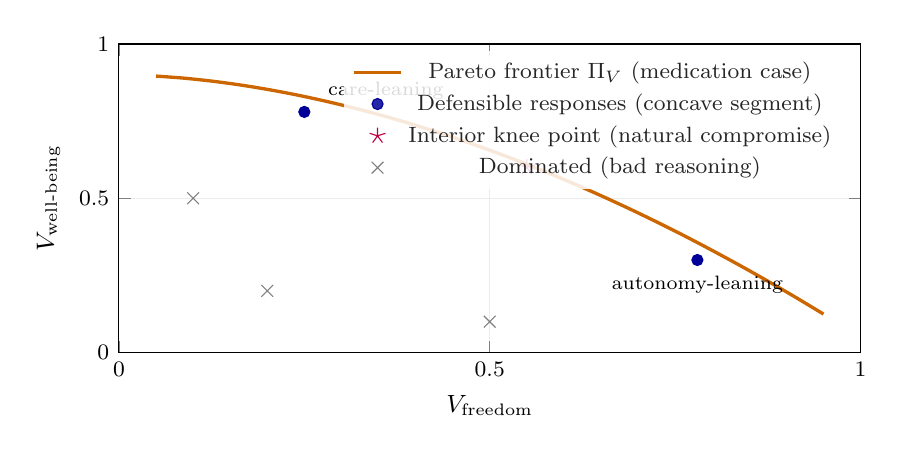
\begin{tikzpicture}
    \begin{axis}[
      width=11cm, height=5.5cm,
      xlabel={$V_{\text{freedom}}$}, ylabel={$V_{\text{well-being}}$},
      xmin=0, xmax=1, ymin=0, ymax=1,
      xtick={0, 0.5, 1.0}, ytick={0, 0.5, 1.0},
      tick label style={font=\footnotesize}, label style={font=\small},
      grid=both, grid style={gray!15},
      legend style={font=\footnotesize, at={(0.98,0.98)}, anchor=north east,
        draw=none, fill=white, fill opacity=0.85},
    ]
      \addplot[orange!80!black, very thick, smooth, domain=0.05:0.95]
        {0.9 - 0.85*x^1.8};
      \addlegendentry{Pareto frontier $\Pi_V$ (medication case)}
      \addplot[only marks, mark=*, mark size=2pt, blue!60!black] coordinates {
        (0.78, 0.30) (0.25, 0.78)
      };
      \addlegendentry{Defensible responses (concave segment)}
      \addplot[only marks, mark=star, mark size=3pt, purple] coordinates {(0.55, 0.60)};
      \addlegendentry{Interior knee point (natural compromise)}
      \addplot[only marks, mark=x, mark size=3pt, gray] coordinates {
        (0.2, 0.2) (0.5, 0.1) (0.1, 0.5)
      };
      \addlegendentry{Dominated (bad reasoning)}
      \node[font=\scriptsize] at (axis cs:0.78, 0.22) {autonomy-leaning};
      \node[font=\scriptsize] at (axis cs:0.36, 0.85) {care-leaning};
    \end{axis}
  \end{tikzpicture}
  \caption{Sketch of the ethical-value Pareto frontier in the medication
    case, projected onto \textsc{freedom} and \textsc{well-being}. Two
    defensibly different responses sit on a concave segment; an interior
    knee point captures a natural compromise; several reachable responses
    are strictly dominated.}
  \label{fig:medication-landscape}
\end{figure}


\section{Strategies for navigating the space}
\label{sec:strategies}

If moral reasoning aims at the frontier, the natural follow-up question is
\emph{how an agent gets there}. Reflective equilibrium is the
philosopher-favoured answer, but it is one strategy among several. We
sketch the space of strategies and the primitives they share.

\paragraph{Shared primitives.} Any strategy that walks toward $\Pi$ requires
three capacities, independent of how those capacities are combined:
\emph{principle proposal} (induction from commitments to a candidate
principle), \emph{principle deduction} (derivation of commitments implied
by a principle), and \emph{coherence checking} (assessment of $\sigma$ on
the epistemic and ethical axes). For an artificial moral reasoner, these
are the capacities to evaluate.

\paragraph{Reflective equilibrium.} Beginning from the initial commitments
$C_0$ and an arbitrary $T$, alternate revisions of $T$ and $C$, each step
guided by current scores~\citep{beisbart2021}. The trace is local: each move
depends on the current state, and the trajectory walks toward a fixed point.
Reflective equilibrium is well-suited to finite reasoners with strong
intuitions and limited search budget; it is the canonical strategy in the
philosophical literature.

\paragraph{Sample-and-prune.} Generate many candidate epistemic states by
combining principles and commitments, score each, retain the non-dominated
ones. A direct attempt to map a region of $\Pi$ rather than walk toward a
single point. Well-suited to reasoners with cheap sampling, perhaps less
well-suited to finite human deliberation.

\paragraph{Tree search.} Build a tree of reasoning moves from $\sigma_0$,
expand promising branches, backtrack from dead ends. A natural fit for
artificial reasoners with a notion of branch quality and a backtracking
mechanism.

\paragraph{Single-pass abduction.} Propose one principle from $C_0$, deduce
its consequences, accept the result. The naive baseline. Often
under-evaluated against the others.

\paragraph{Multi-start equilibrium.} Run reflective equilibrium from several
distinct starting points to discover multiple regions of $\Pi$ at once.
Particularly useful when the frontier is expected to be concave or
plateau-shaped.

\paragraph{Corner-collapse strategies.} Maximise a single axis (pure
\textsc{Account}, pure \textsc{welfare}, pure \textsc{autonomy}). Degenerate
in general but instructive as ablations and as failure modes of stronger
strategies.

\paragraph{Which strategy for which reasoner?} For humans, reflective
equilibrium is the canonical answer, in part because human deliberation has
a budget that favours local moves over wide sampling. For artificial
reasoners --- LLMs in particular --- the question is open. Sampling-based
strategies may exploit parallelism that humans cannot; tree-search
strategies may map richer landscapes; the failure modes of single-pass
strategies may or may not appear under chain-of-thought. The framework lets
us ask these questions on equal footing once we can locate any strategy's
output in the space.


\section{A corpus to make this empirical}
\label{sec:corpus}

The framework so far is conceptual; turning it empirical requires a corpus.
We sketch what we would dream of having and what it would let us do.

\paragraph{Contents.} For a body of ethical situations, the corpus would
contain three layers.

\begin{enumerate}[leftmargin=*, itemsep=2pt]
  \item \textbf{Commitment pool} $\mathcal{C}$: candidate verdicts on each
    situation. Per-case action judgments of the form ``in situation $s$,
    action $a$ is required / permissible / forbidden,'' generated broadly
    enough to cover the defensible verdicts plus a margin of bad ones.
  \item \textbf{Principle pool} $\mathcal{P}$: candidate moral principles,
    each tagged with a \emph{fuzzy value loading} $\boldsymbol{v}(p) \in [0,1]^K$
    indicating to what degree the principle expresses each value. Optionally,
    a secondary tagging by ethical framework $\boldsymbol{f}(p) \in [0, 1]^M$
    (utilitarian, Kantian, virtue, care, contractualist) supports
    framework-level analyses without committing to frameworks as primary
    axes.
  \item \textbf{Dialectical graph} $\rho$: for every principle-commitment
    pair, a \emph{fuzzy inferential strength}
    $\rho(p, c) \in [-1, 1]$, where positive values indicate degree of
    entailment, negative values degree of contradiction, and zero
    silence. This generalises a discrete entails / contradicts / silent
    labelling and captures the partial support relations that are typical
    in moral reasoning.
\end{enumerate}

\paragraph{Construction.} The corpus would be generated by a large language
model and verified by philosophers at every stage --- generation, fusion of
near-duplicates, deletion of weak candidates, scoring of independent
quality dimensions, value tagging, and inferential strengths. We treat the
corpus as a reusable resource in its own right, independent of any
downstream reasoning method that operates on it.

\paragraph{What it would let us do.} Given a starting set of intuitions
$C_0$ drawn from $\mathcal{C}$, the corpus lets us:

\begin{itemize}[leftmargin=*, itemsep=2pt]
  \item Compute the Pareto fronts $\Pi_E$ and $\Pi_V$ of attainable
    epistemic states, and characterise their shapes locally and globally.
  \item Locate any epistemic state $\sigma$ in the joint space, and say
    whether it is on $\Pi$, near $\Pi$, or dominated --- and if dominated,
    by what.
  \item Inspect reasoning traces move by move: is each step principled
    (a justified abduction, a defensible commitment revision) or
    unprincipled (a faithfulness violation with no compensating gain)?
    Does the trajectory walk toward $\Pi$ or away from it?
  \item Compare reasoning strategies on equal footing.
\end{itemize}


\section{What this lets us study}
\label{sec:study}

The framework, combined with such a corpus, opens several lines of empirical
work that are difficult to pose otherwise.

\paragraph{The geometry of moral disagreement.} For a given case, is the
local shape of $\Pi$ convex (resolvable disagreement) or concave (genuine
pluralism)? Does the case admit a knee point (a natural compromise)? Across
many cases, what shapes recur, and what does that tell us about the
structure of the moral domain?

\paragraph{Strategy comparison.} Do different reasoning strategies reach
different regions of $\Pi$ on the same case? Does reflective equilibrium
land in plateaus while sample-and-prune maps concave segments? Which
strategy is more robust under reframing of the case?

\paragraph{LLM moral reasoning.} A value-aligned model whose traces sit
off $\Pi$ in characteristic ways is a value-aligned model that reasons
badly --- and the framework lets us name how. Specific failure modes
become diagnosable: \emph{corner collapse} (the trace ends at an axis
extreme), \emph{anti-revision rigidity} (no move revises the principle
side), \emph{faithfulness violations} (commitments dropped with no
justifying gain), \emph{stability collapse} (different landings under
semantically equivalent rephrasings of the situation). These are
empirically testable hypotheses about LLM behaviour, but they only become
testable once the framework names them.

\paragraph{The capacities that matter.} If the shared primitives of
Section~\ref{sec:strategies} are the irreducible capacities of moral
reasoning, then the question for any artificial moral reasoner is: which
of those capacities does it have, and at what quality? The corpus lets us
isolate each primitive --- principle proposal, principle deduction,
coherence checking --- and evaluate it independently of the strategy it is
embedded in.


\section{Discussion}
\label{sec:discussion}

We have argued that moral reasoning is best framed not as the search for a
single right answer but as navigation of a multi-objective landscape whose
Pareto frontier is the space of defensible answers. The framework gives
familiar pieces a clearer place: the goal of moral reasoning is a good
epistemic state; goodness is graded along epistemic and ethical axes that
genuinely conflict; the rational object of study is the Pareto frontier of
attainable states; reasoning methods such as reflective equilibrium are
strategies for navigating this landscape, alongside other strategies that
may suit artificial reasoners better. The descriptive vocabulary of
multi-objective optimisation lets us name what we see: convex and concave
segments, knee points, plateaus, corner attractors, dominated regions ---
and the failure modes of reasoners that get stuck in any of them.

The work the framework still requires is the corpus
(Section~\ref{sec:corpus}) and the empirical study it would support
(Section~\ref{sec:study}). Neither is small, but both are now well-posed:
the framework tells us what to build and what to measure.


\begin{thebibliography}{9}

\bibitem[Beisbart et~al.(2021)]{beisbart2021}
Claus Beisbart, Gregor Betz, and Georg Brun.
\newblock Making reflective equilibrium precise: A formal model.
\newblock \emph{Ergo}, 8(15):441--472, 2021.

\bibitem[Carlsmith(2026)]{carlsmith2026}
Joe Carlsmith.
\newblock How do we solve the alignment problem?
\newblock Essay series, 2026.
\newblock \url{https://joecarlsmith.com/}.

\bibitem[Deb(2001)]{deb2001multiobjective}
Kalyanmoy Deb.
\newblock \emph{Multi-Objective Optimization Using Evolutionary Algorithms}.
\newblock John Wiley \& Sons, 2001.

\bibitem[Queloz(2025)]{queloz2025}
Matthieu Queloz.
\newblock Can AI rely on the systematicity of truth? The challenge of modelling
  normative domains.
\newblock \emph{Philosophy \& Technology}, 38(1):34, 2025.

\bibitem[Rawls(1971)]{rawls1971}
John Rawls.
\newblock \emph{A Theory of Justice}.
\newblock Harvard University Press, 1971.

\end{thebibliography}

\end{document}
